\documentclass[ti]{texufpel} %use tid para doutorado e ti para mestrado

\usepackage[utf8]{inputenc} % acentuacao
\usepackage{graphicx} % para inserir figuras
\usepackage[T1]{fontenc}
\usepackage{todo}
\usepackage{amssymb}

\hypersetup{
    hidelinks, % Remove coloração e caixas
    unicode=true,   %Permite acentuação no bookmark
    linktoc=all %Habilita link no nome e página do sumário
}

\unidade{Centro de Desenvolvimento Tecnológico}
\programa{Programa de Pós-Graduação em Computação}
\curso{Ciência da Computação}

\title{Memórias Transacionais}

\author{Costa}{Michael Alexandre}
\advisor[Prof.~Dr.]{Du Bois}{André Rauber}
\coadvisor[Prof.~Dr.]{Pilla}{Mauricio Lima}


%Palavras-chave em PT_BR
\keyword{Memótia Transacional}
\keyword{NUMA}
\keyword{UMA}
\keyword{Escalonamento}

%Palavras-chave em EN_US
\keywordeng{Transacional Memory}
\keywordeng{NUMA}
\keywordeng{UMA}
\keywordeng{Scheduler}

\begin{document}


\maketitle

\sloppy

%Resumo em Portugues (no maximo 500 palavras)
\begin{abstract}
  ...
\end{abstract}

\begin{englishabstract}%
  {Transacional Memory}% {Titulo do Trabalho em Ingles}

  ...
\end{englishabstract}

%Lista de Figuras
\listoffigures

%Lista de Tabelas
\listoftables

%lista de abreviaturas e siglas
\begin{listofabbrv}{SPMD}
        \item[ATS] Adaptive Transactional Scheduling
        \item[STM] Software Transactional Memory
        \item[TM] Transactional Memory
        \item[NUMA] Non-Uniform Memory Access
\end{listofabbrv}

%Sumario
\tableofcontents

\chapter{Introdução}

 ...

\section{Uma subseção}

  ...

%---------------------------------------------------------------------------------------------------%
%---------------------------------------------------------------------------------------------------%
\chapter{Memória Transacional}

Memória Transacional, ou \emph{Transactional Memory}~(TM), é uma classe de mecanismos de sincronização que fornece uma execução atômica e isolada de alterações em um conjunto de dados compartilhados. Estas estão sendo desenvolvidas para que no futuro tornem-se o principal meio de fazer a sincronização em um programa concorrente, substituindo a sincronização baseada em \emph{locks}~\cite{herlihy06}. As TMs podem ser implementadas em \emph{software} (STM), em \emph{hardware} (HTM) ou ainda em uma versão híbrida de \emph{hardware} e \emph{software}.

Na programação utilizando STMs, todo o acesso à memória compartilhada é realizado dentro de transações e todas as transações são executadas atomicamente em relação a transações concorrentes.

A principal vantagem na programação usando STM é que o programador apenas delimita as seções criticas e não é necessário preocupar-se com a aquisição e liberação de \emph{locks}. Os \emph{locks}, quando utilizados de forma incorreta, podem levar a problemas como \emph{deadlocks}~\cite{bandeira10}.

%---------------------------------------------------------------------------------------------------%
\section{Propriedades}

Transação é uma sequência finita de escritas e leituras na memória executada por uma \emph{thread}~\cite{herlihy93}, e deve satisfazer três propriedades:

\begin{itemize}
 \item \textbf{Atomicidade}: cada transação faz uma sequência de mudanças provisórias na memória compartilhada. Quando a transação é concluída, pode ocorrer um \emph{commit}, tornando suas mudanças visíveis a outras \emph{threads} instantaneamente, ou pode ocorrer um \emph{abort}, fazendo com que suas alterações sejam descartadas;

 \item \textbf{Consistência}: as transações devem garantir que um sistema consistente deve ser mantido consistente. Esta propriedade esta relacionada com o conceito de invariância;

 \item \textbf{Isolamento}: as transações não interferem nas execuções de outras transações, assim parecendo que elas são executadas serialmente. Uma transação não observa o estado intermediário de outra.
\end{itemize}

%---------------------------------------------------------------------------------------------------%
\section{Versionamento de Dados}

O versionamento de dados faz é responsável pelo gerenciamento das versões dos dados. Ele armazena tanto o valor do dado no início de uma transação como também o valor do dado modificado durante a transação, isso para garantir a propriedade de atomicidade~\cite{baldassinTese09}.

\begin{figure}[!htp]
\centering
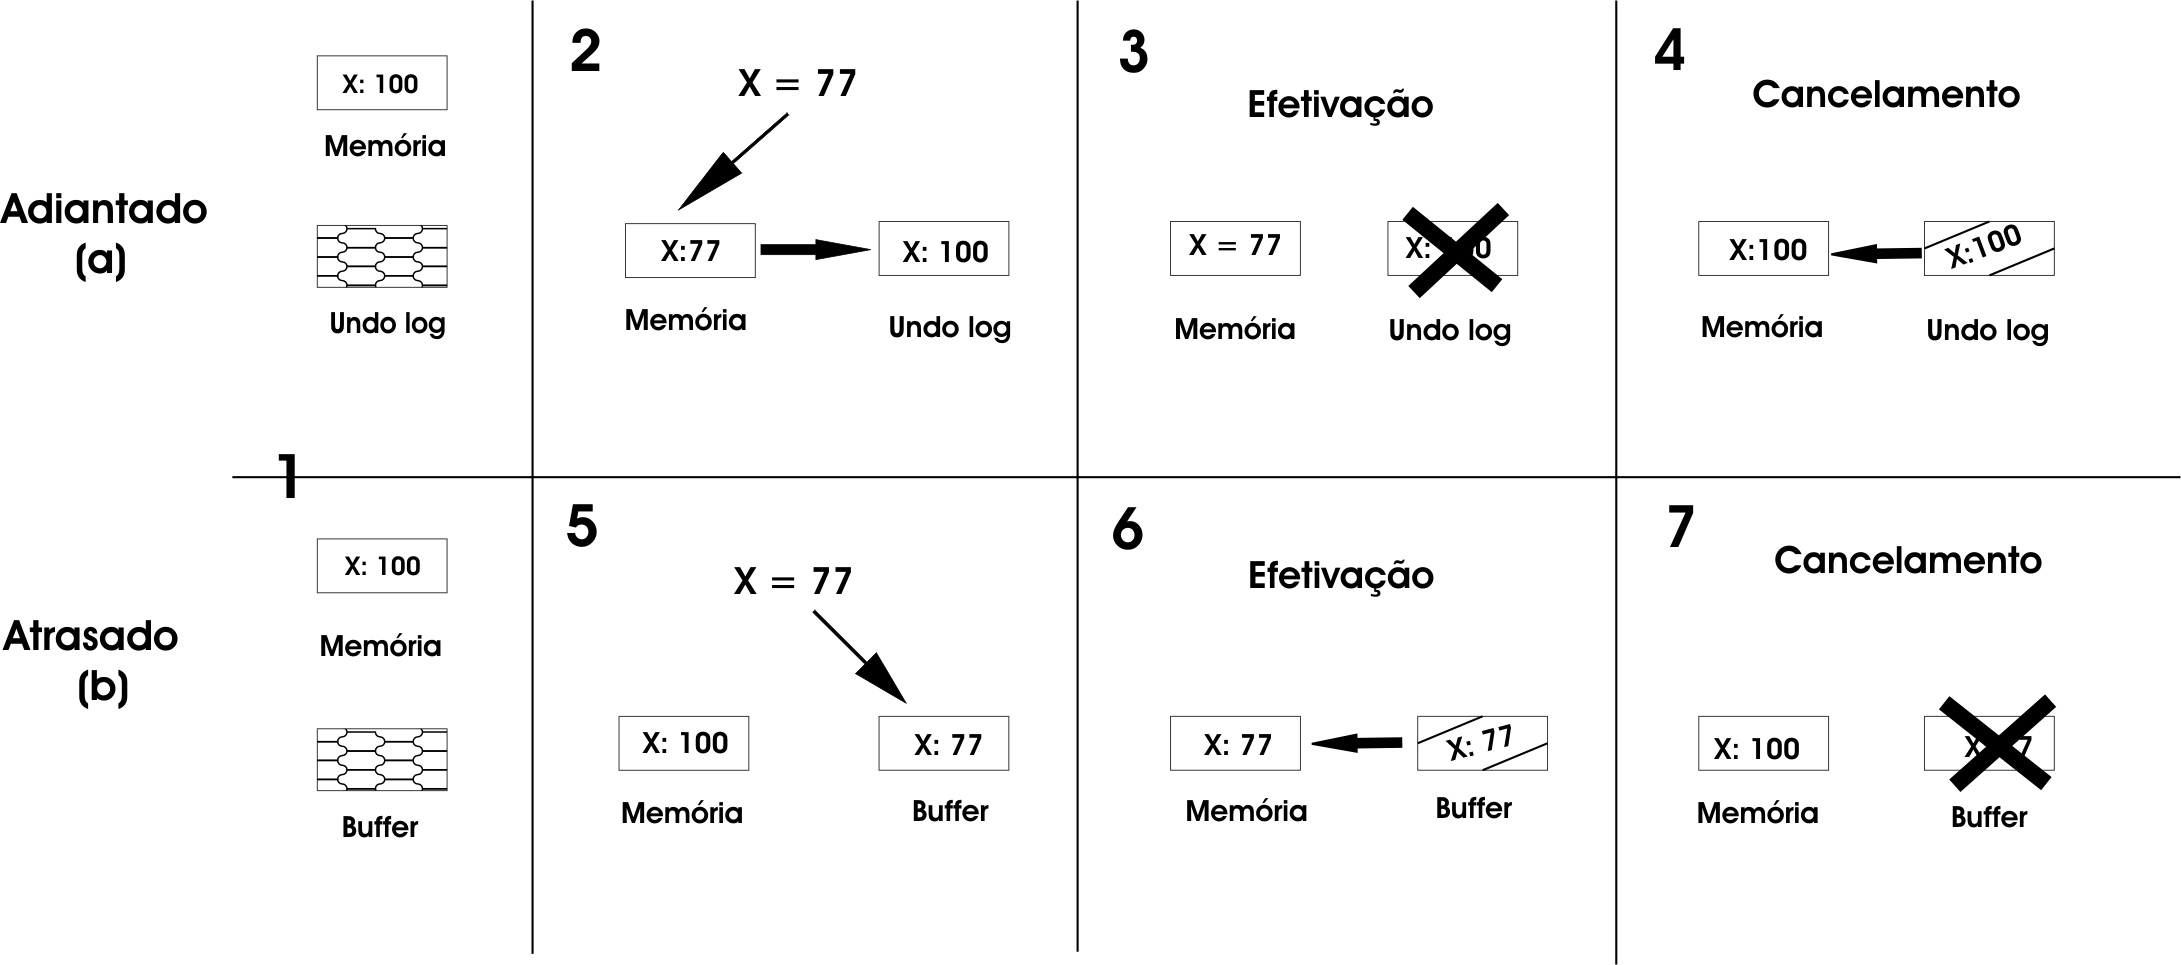
\includegraphics[height=7cm]{Imagens/versionamento.png}
\caption{Exemplo de versionamento adiantado (a) e atrasado (b). Fonte:~\cite{baldassinTese09}}
\label{figuraVersionamento}
\end{figure}

Existem dois tipos de versionamento de dados:

\begin{itemize}
 \item \textbf{Versionamento Adiantado}: como pode ser visto na Figura~\ref{figuraVersionamento}~(a), o valor modificado durante a transação é armazenado direto na memória e o valor inicial é armazenado em um \emph{undo log}, para que no caso de cancelamento na transação o valor inicial seja restaurado na memória.

 \item \textbf{Versionamento Atrasado}: como pode ser visto na Figura~\ref{figuraVersionamento}~(b) neste versionamento o valor modificado durante a transação é armazenado em um \emph{buffer} e o valor inicial é mantido na memória até que aconteça um \emph{commit} na transação, onde o valor armazenado no \emph{buffer} é escrito na memória. Caso aconteça o cancelamento na transação, o valor do \emph{buffer} é descartado.
\end{itemize}

%---------------------------------------------------------------------------------------------------%
\section{Detecção de Conflito}

Mecanismos de detecção de conflitos verificam a existência de operações conflitantes durante uma transação. Um conflito ocorre quando duas transações estão acessando um mesmo dado na memória e pelo menos uma das transações está fazendo uma operação de escrita~\cite{baldassinTese09}.

Da mesma forma que o versionamento de dados, a detecção de conflito também pode ser de dois tipos:

\begin{itemize}
 \item \textbf{Detecção de Conflitos Adiantado}: ocorrem no momento em que duas transações acessam um mesmo dado e uma delas faz uma operação de escrita. Essa operação de escrita é detectada e então uma transação é abortada. Neste tipo de detecção pode ocorrer o problema chamado de \emph{livelock}, quando duas transações ficam cancelando-se, desta forma, a execução do programa não progride. A Figura~\ref{figuradeteccaoadiantado} mostra como é feita a detecção de conflitos adiantado.

 O Caso~1, mostra a execução sem conflitos, onde as duas transações são executadas sem problemas. Já o Caso~2, mostra o que acontece quando ocorre um conflito, onde T1 lê A e logo depois T2 escreve em A, então o conflito é detectado e T1 é abortada, após ser efetivada T2, a transação T1 consegue ler A sem problema de conflito. Por fim o Caso~3 mostra a situação de \emph{livelock}, onde as duas transações tentam ler e escrever em A, assim as duas acabam sempre se abortando.

\begin{figure}[!htp]
\centering
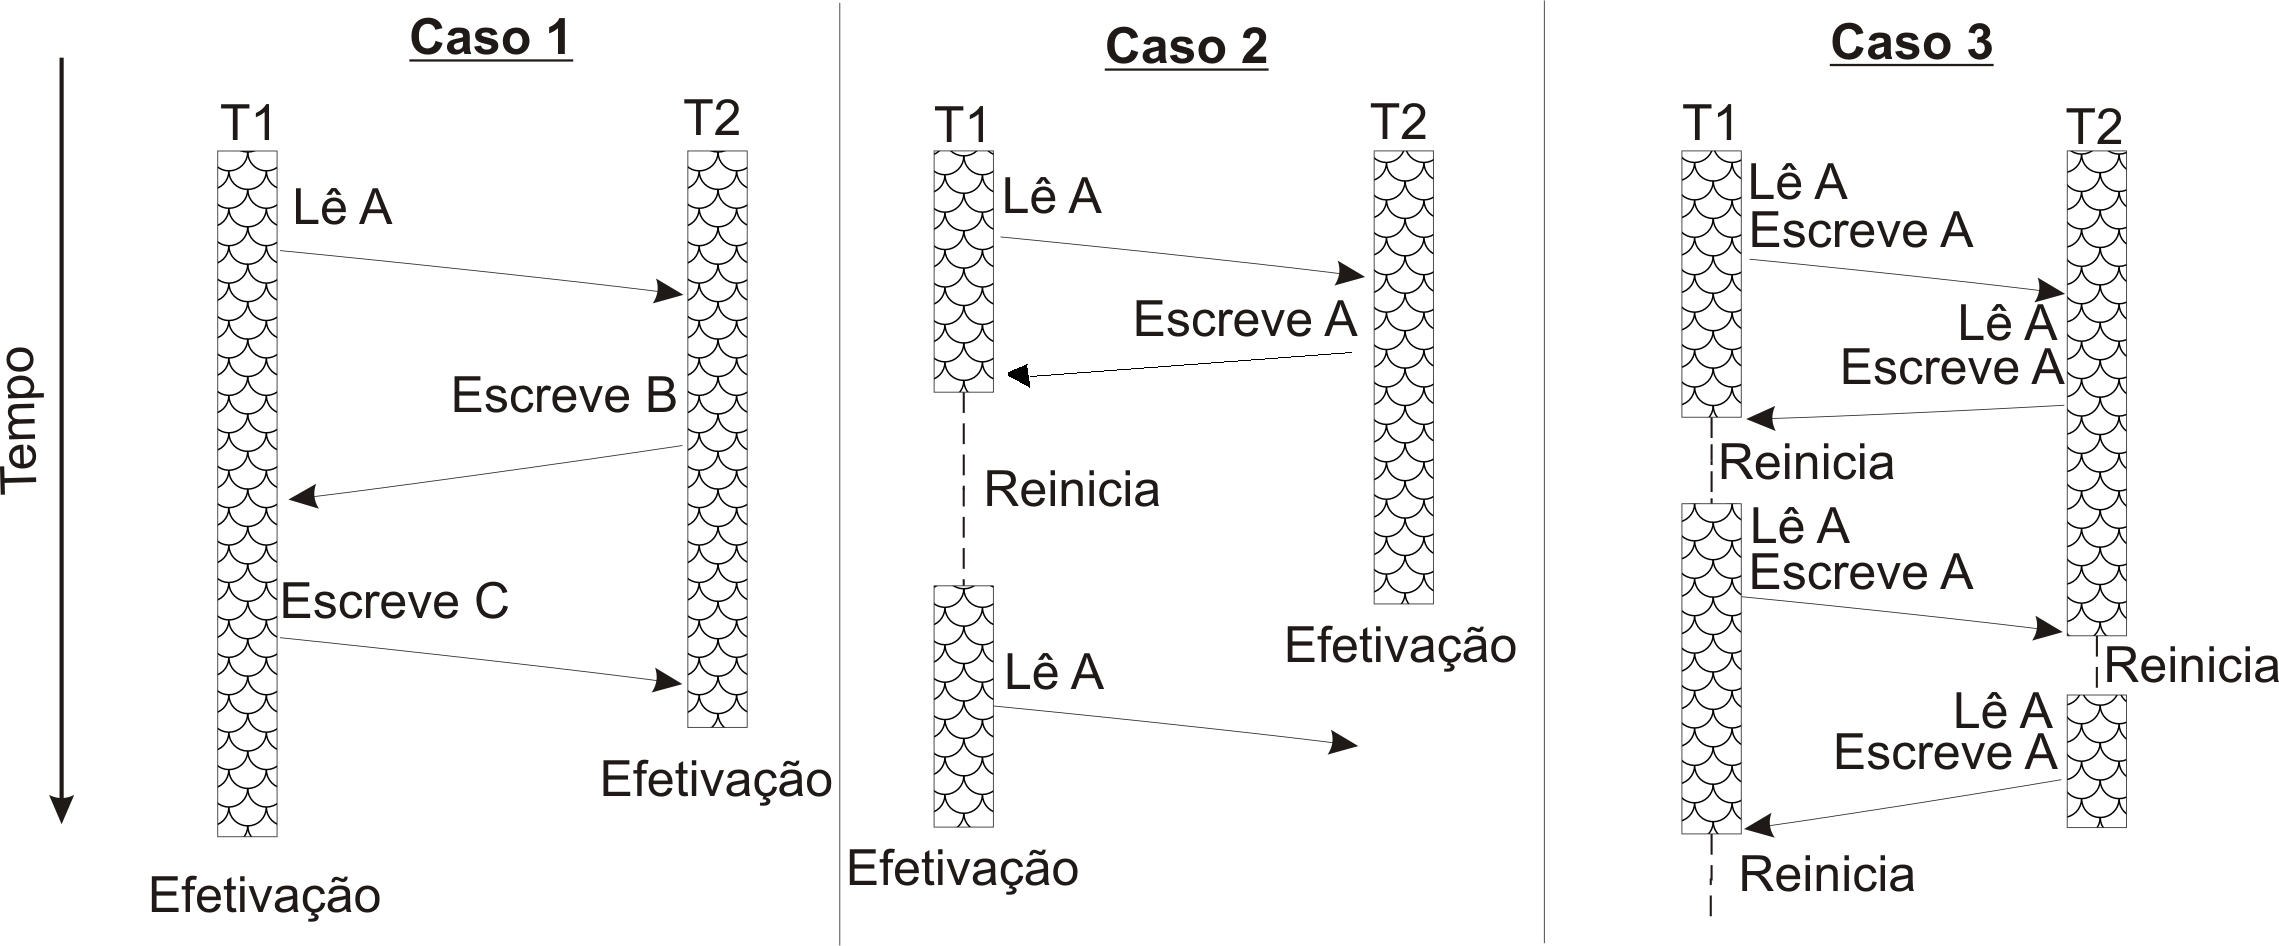
\includegraphics[height=6.5cm]{Imagens/conflitoadiantado.png}
\caption{Detecção de conflitos em modo adiantado. Fonte:~\cite{rigo07}}
\label{figuradeteccaoadiantado}
\end{figure}

 \item \textbf{Detecção de Conflitos Atrasado}: Este tipo de detecção de conflito ocorre no final da transação.  Antes da transação ser efetuada, é verificado se ocorreu um conflito. Caso tenha ocorrido, a transação é cancelada, senão é efetivada. Para transações muito grandes não é recomendado este tipo de detecção, pois uma transação grande pode ser abortada várias vezes por transações pequenas, assim gastando tempo de processamento desnecessário, este problema se chama \emph{starvation}. A Figura~\ref{figuradeteccaoatrasado} mostra como é feita a detecção de conflitos atrasado.

 O Caso~1, mostra as transações acessando dados diferentes, não ocasionando conflitos. No Caso~2, T2 lê A que é escrita por T1. A T2 só nota o conflito quando T1 é efetivado. Logo depois de notar o conflito T2 é abortada. No Caso~3 não ocorre nenhum conflito, pois T1 lê A antes de T2 escrever. O Caso~4 mostra a situação em que, após ser cancelada, T1 volta a executar.
\end{itemize}

\begin{figure}[!htp]
\centering
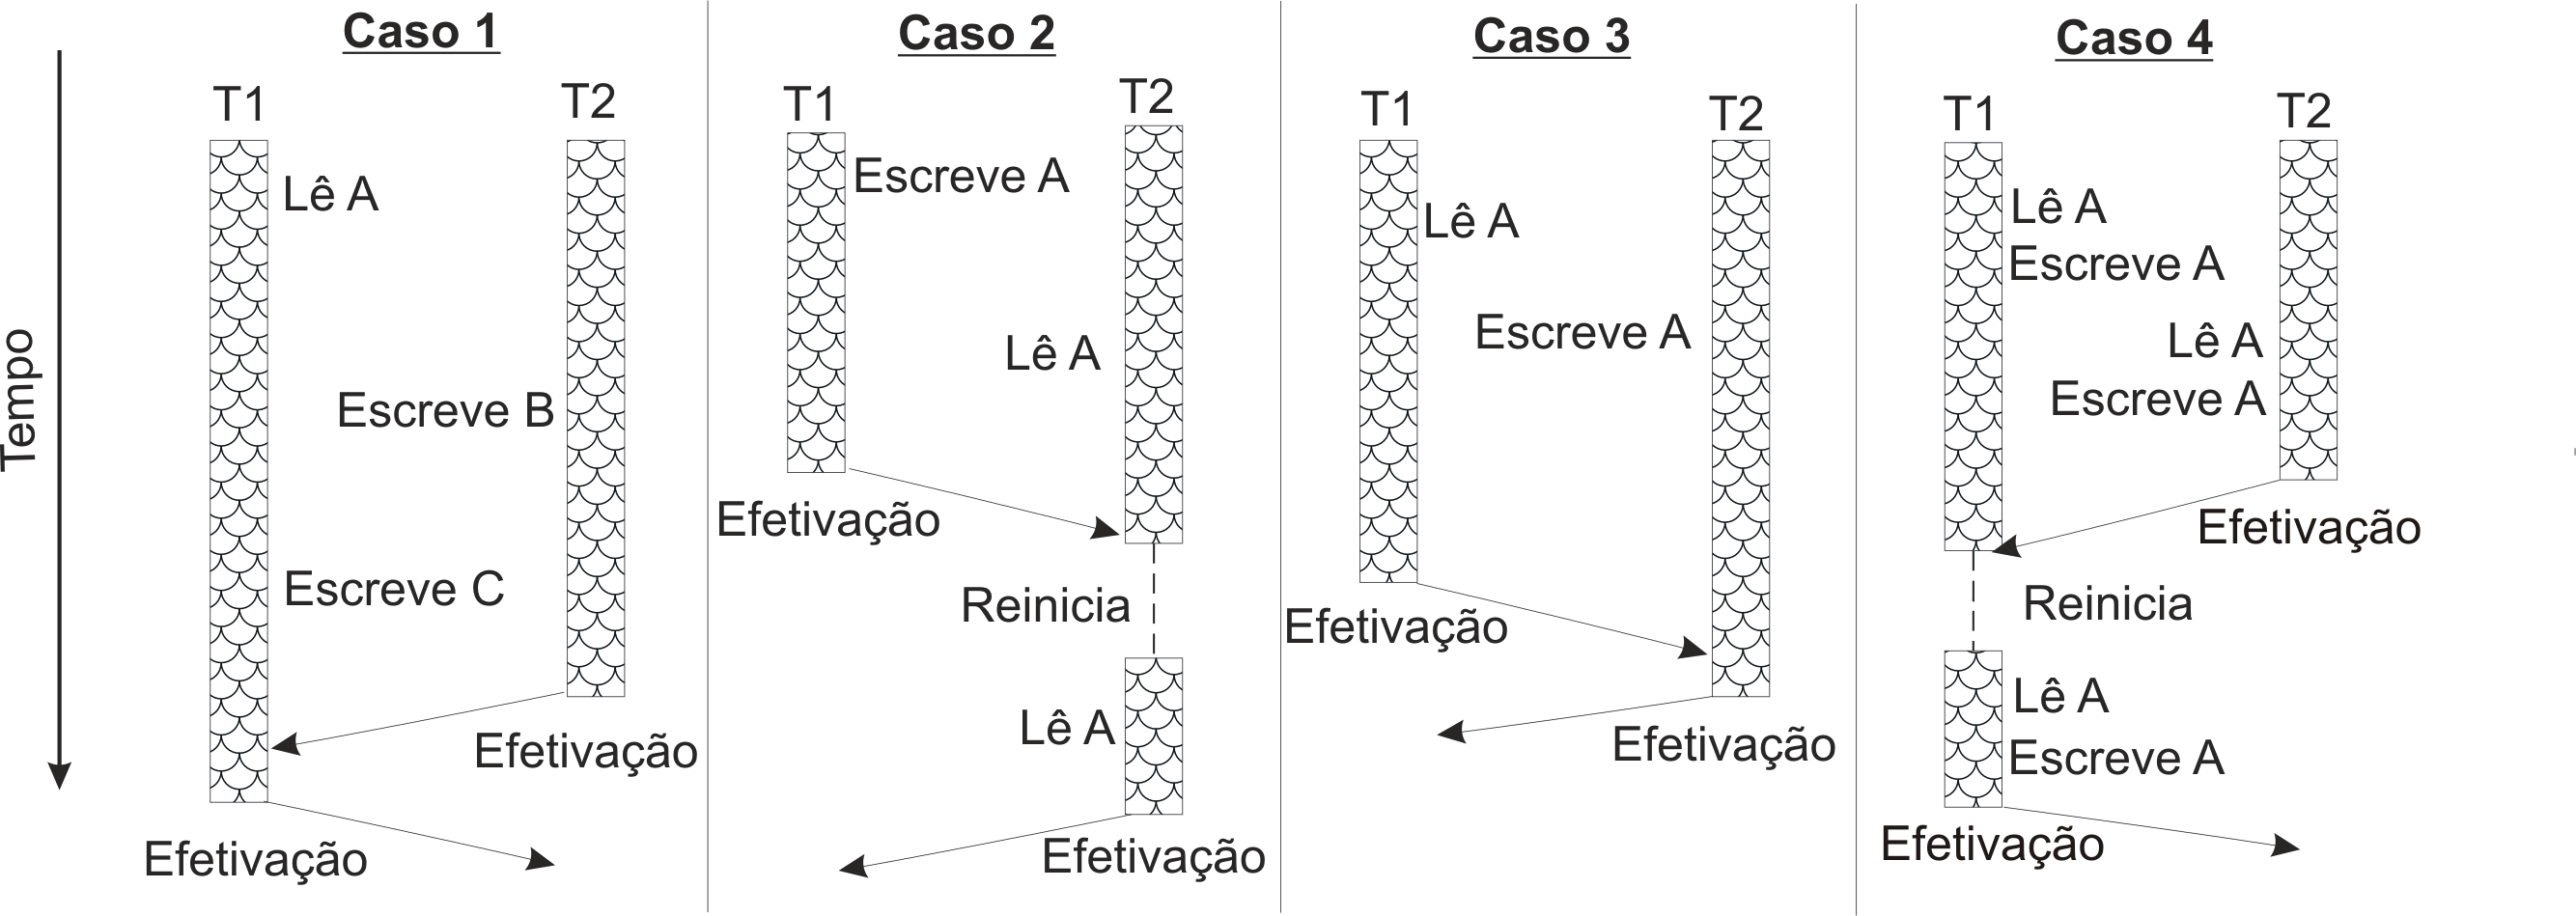
\includegraphics[height=6.5cm]{Imagens/conflitoatrasado.png}
\caption{Detecção de conflitos em modo atrasado. Fonte:~\cite{rigo07}}
\label{figuradeteccaoatrasado}
\end{figure}

Para solucionar o problema de qual transação continuará executando, quando ocorre um conflito, é utilizado um gerenciador de contenção~\cite{harris10}. O gerenciador de contenção é o responsável por decidir quando e qual transação vai ser abortada, isso para garantir que a execução do programa prossiga sem problemas.

%---------------------------------------------------------------------------------------------------%
%---------------------------------------------------------------------------------------------------%
\chapter{Escalonamento de STM}

  A bibliografia de STM apresenta um gama distinta e extensa de estratégias de escalonamento. Estas diferem-se devido as distintas características de aplicações encontradas. Nas quais podem apresentar maior ou menor nível de contenção, diferentes read-sets e write-sets, entre outras características.

  Os algoritmos de escalonamento visam otimizar o tempo de execução. Para isto devem inserir o menor \emph{overhead} possível no código propondo uma estratégia eficiente para as características do problema abordado. Alguns algoritmos estudados, como \emph{CAR-STM}~\cite{dolev08}, buscam serializar transações conflitantes com a utilização de filas de transações.

  Os escalonadores de STM estudados na bibliografia caracterizam-se por executar o escalonamento em dois níveis distintos. Os dois níveis buscam reduzir o tempo de execução e garantir a execução do programa. Estes escalonamentos de STM são o escalonamento de \emph{threads} e de transações.

  O escalonamento de \emph{threads}, busca executar sua tomada de decisão sobre as \emph{threads} ativas no programa, podendo adicionar mais \emph{threads}, remove-las, ou migra-las entre os \emph{cores}.

  O escalonamento de transações, busca executar sua tomada de decisão sobre as transações do programa, estas podem estar em execução, já terem sido abortadas, ou serem a próxima a executar.

  As tomadas de decisões dos escalonadores citados acima se dá a partir de outras características. Estas avaliam de forma diferente os dados para a tomada de decisão e em tempos de execução diferentes, assim como, podem efetuar operações distintas conforme suas premissas de escalonamento.

\section{Características e Técnicas}

O trabalho \cite{sanzo17}, classifica as técnicas de escalonamento de STM como, baseadas em heurísticas e baseadas em modelos, esta classificação é apresentada na Figura~\ref{figuraCategoria}, onde cada classe, apresenta técnicas distintas de escalonamento.

Estas diferentes técnicas apresentadas foram exploradas e exemplificadas no trabalho citado acima. As subseções a seguir vão abordar e detalhar estas técnicas, assim como seus algoritmos.

\begin{figure}[!htp]
\centering
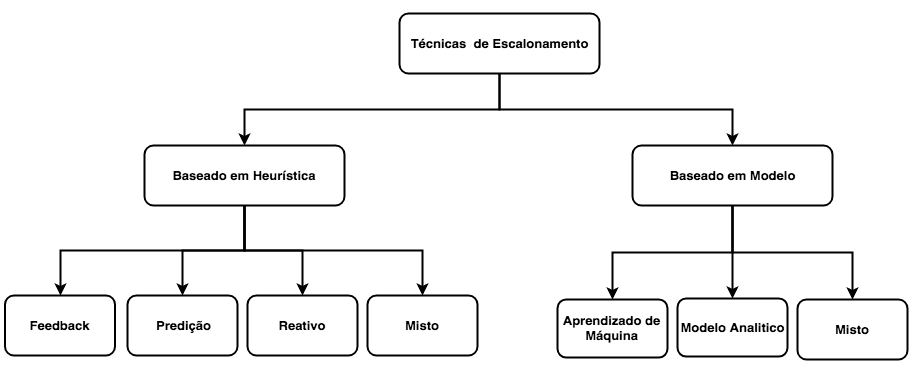
\includegraphics[height=6.5cm]{Imagens/categoriasEscalonamento.png}
\caption{Classificação das técnicas de escalonamento. Fonte:~\cite{sanzo17}}
\label{figuraCategoria}
\end{figure}

\subsection{Técnica baseada em Feedback}

As técnicas baseadas em feedback utilizam um sistema de loop fechado para controle de um sistema dinâmico. Essa técnica utiliza um parâmetro de desempenho que é avaliado pelo escalonador a cada iteração do loop para decidir a ação a ser executada, um exemplo de escalonador baseado em feedback é denominado \emph{Adaptive Transactional Scheduling} (ATS).

O escalonador ATS, apresentado em \cite{yoo08}, tem como objetivo otimizar a execução de código e reduzir o número de conflitos por meio da serialização das transações conflitantes. Para serializar as transações o escalonador utiliza uma fila de compartilhamento global.

O escalonador toma a decisão de serializar ou não uma transação conflitante utilizando um parâmetro de feedback denominado \emph{Contention Intensity} (CI). Cada \emph{thread} em execução possui um CI, que é calculado individualmente por uma média dinâmica, este cálculo é efetuado quando uma transação é anulada ou confirmada. A função que calcula o CI é: $CI = \alpha * CIprev + (1 - \alpha) * CC$.

Onde $CIprev$ é o valor anterior a $CI$, $CC$ é igual a 0 se a transação for anulada e igual a 1 se a transação for confirmada, $\alpha$ possui um valor entre 0 e 1, e afeta o peso histórico das transações do \emph{thread}.

Quando um $CI$ ultrapassa o limite previamente definido, o escalonador toma a decisão de serializar as transações executadas por este \emph{thread} em relação às transações executadas por outro \emph{thread}, inserindo então as transações na fila de compartilhamento global.


\subsection{Técnica baseada em Previsão}

As técnicas baseadas em previsão utilizam probabilidade para tomar a decisão apropriada para sua execução. Essa técnica utiliza um conjunto de dados de um mesmo parâmetro para estimar a probabilidade de execução, assim o escalonador toma a decisão de execução dinamicamente. Um exemplo de escalonador baseado em previsão é denominado \emph{Shrink}.

O escalonador \emph{Shrink}, apresentado em \cite{dragojevic09}, utiliza a suposição de localidade temporal e serializa as transações se os conjuntos de dados previstos mostrarem que um conflito pode ocorrer.

Para isto, é utilizado como base, os dados lidos pelas n transações executadas por um \emph{thread}. Este conjunto de leitura de uma transação utiliza o valor n como uma janela de localidade.

Assim, se um item de dados tiver sido lido pela transação anterior, é incrementado, com uma constante de confiança (CI), o parâmetro confiança (C). Se este ultrapassar o limite de confiança estipulado, o item de dados é adicionado ao conjunto de leitura previsto.

O conjunto de gravação é previsto apenas para reiniciar as transações, presumindo-se que este inclua dados pertencentes ao conjunto de gravação da última transação anulada.

Visando reduzir o \emph{overhead} de execução, o escalonador \emph{Shrink} entra em ação para um \emph{thread} apenas quando sua taxa de sucesso de transação está abaixo de um limite de sucesso.


\subsection{Técnicas Reativas}

As técnicas reativas adotam uma estratégia onde o escalonador entra em ação após uma transação ser abortada, isso busca evitar conflitos repetidos. Esta estratégia baseia-se na suposição de que os dados acessados por uma transação abortada tem a possibilidade de serem os mesmos acessados durante sua reexecução, ocasionando novo conflito com a transação ainda em execução. Um exemplo de escalonador que utiliza técnicas reativas é conhecido como \emph{CAR-STM}.

O escalonador \emph{CAR-STM}, apresentado em \cite{dolev08}, apresenta duas políticas. A primeira, denominada \emph{Basic Seraling Contention Management}~(DSCM), reduz a probabilidade de duas transações, que já conflitaram, conflitem novamente. A segunda política, denominada \emph{Gerenciamento de Prevenção de Serialização Permanente}~(PSCM), garante que duas transações conflitantes nunca conflitem novamente.

Com a política PSCM, se uma transação \emph{A} entrar em conflito com uma transação \emph{B} e \emph{A} for iniciada após \emph{B}, \emph{A} será abortada. A transação abortada é colocada na fila de execução da \emph{thread} na qual a transação conflitante pertence. Isso reduz a probabilidade de ocorrer novamente um conflito entre estas transações.

Ainda há a possibilidade de ocorrer um conflito entre estas transações. Se \emph{B} conflitar com uma terceira transação, então \emph{B} será colocada em uma fila de transação que será executado por outro \emph{thread}, assim, permitindo novamente um conflito com \emph{A}. Para evitar esta situação, a política PSCM, marca transação abortada como subordinada a transação conflitante, assim, caso a transação conflitante for movida de fila, as transações subordinadas a esta serão movidas junto.

O \emph{CAR-STM} também possui a opção de escalonamento proativo, onde o escalonador não precisa que um conflito ocorra. Neste caso, o escalonador possui informações sobre a possibilidade de conflito entre pares de transações. Estas informações são fornecidas ao escalonador pela aplicação utilizada, deixando a cargo do desenvolver a tarefa de manter o escalonador ciente dos acessos realizados pelas transações.

\subsection{Técnica baseada em Heurística Mista}

As técnicas baseadas em heurísticas mista buscam mesclar as diferentes técnicas comentadas acima, para tirar proveito de diferentes perfis de transações. Assim, o escalonador pode tomar a melhor decisão de execução de acordo com o perfil de execução das transações.  Um exemplo de escalonador que utiliza técnicas reativas é conhecido como \emph{LUTS}.

O escalonador \emph{Lightweight User-Transaction Scheduler}~(LUTS), apresentado em \cite{nicacio13}, permite a modificação de sua estratégia de escalonamento de forma dinâmica, para isto, este avalia a duração das transações. O \emph{LUTS} utiliza um conjunto de \emph{threads}, com tamanho igual ao número de núcleos disponivel na arquitetura em que será utilizado.

As transações são agrupadas por \emph{IDs}, onde, todas as transações geradas pelo mesmo bloco de código possuem o mesmo \emph{ID}. O escalonador utiliza o tempo médio das últimas 100 transações confirmadas. Se o tempo médio estiver abaixo de um limite de tempo pré definido, o escalonador serializa as transações com base na intensidade de contenção, assim como feito no escalonador ATS. Porém, o LUTS mantém o valor de \emph{IC} por \emph{ID} de transação.

Quando a média de transações está acima do limite, o escalonador armazena a probabilidade de conflito para cada \emph{ID} de transação em uma estrutura de dados. Quando uma \emph{thread} fica disponível, o escalonador lê os \emph{IDs} de todas as transações em execução e as informações das estruturas de dados para selecionar a transação com menor probabilidade de conflito. A probabilidade de conflito de um ID é incrementada quando uma transação confirmada e decrementada toda vez que uma transação for abortada.

\subsection{Técnicas baseadas em Aprendizado de Máquina}

As técnicas baseadas em aprendizado de máquina utilizam modelos de desempenho. A partir de um conjunto de dados que representa o perfil das transações, o algoritmo aplica monta uma rede de aprendizado para formular as relações do modelo de desempenho. Assim, o escalonador utiliza o modelo de desempenho como função de entrada para tomada de decisão.

\subsection{Técnicas Baseada em Modelos Analíticos}

As técnicas baseadas em modelos analíticos utilizam modelos construídos por equações matemáticas para tomada de decisão do escalonador. Assim, esta técnica tem como entrada de uma função analitica a base de dados da transação, na qual a saída da função será utilizada para moldar o modelo utilizado.

\subsection{Técnica baseada em Modelos Mistos}

As técnicas baseadas em modelos mistos buscam mesclar as técnicas baseadas em modelo já apresentadas. Essa técnica busca avaliar o comportamento das transações previamente e utilizar estratégias mistas para criar o melhor modelo para o escalonador tomar suas decisões.

\chapter{Escalonadores NUMA}

  ...


\chapter{Escalonamento de Transações aplicado à NUMA}

  ...


\chapter{Discussões}

  ...


\chapter{Conclusão}

  ...

% Bibliografia
% http://liinwww.ira.uka.de/bibliography/index.html
% um site que cataloga no formato bibtex a bibliografia em computacao
%\bibliography{nomedoarquivo.bib} (sem extensao)
%\bibliographystyle{formato.bst} (sem extensao)

\bibliography{bibliografia}
\bibliographystyle{abnt}

% Anexos (Opcional)
\annex
\chapter{Um Anexo}

  ...

\end{document}
